\newpage
\section{конструкторский раздел}
	
	В данном разделе приводится описание алгоритма с помощью idef0. Представлена база дынных в ER (Нотация Чена) и классическая ER. Описан формат данных и способ их передачи от клиента к серверу и обратно. Представлен результат тестирования.
	
\subsection{idef0}
	
	% TODO: \usepackage{graphicx} required
	\begin{figure}[H]
		\centering
		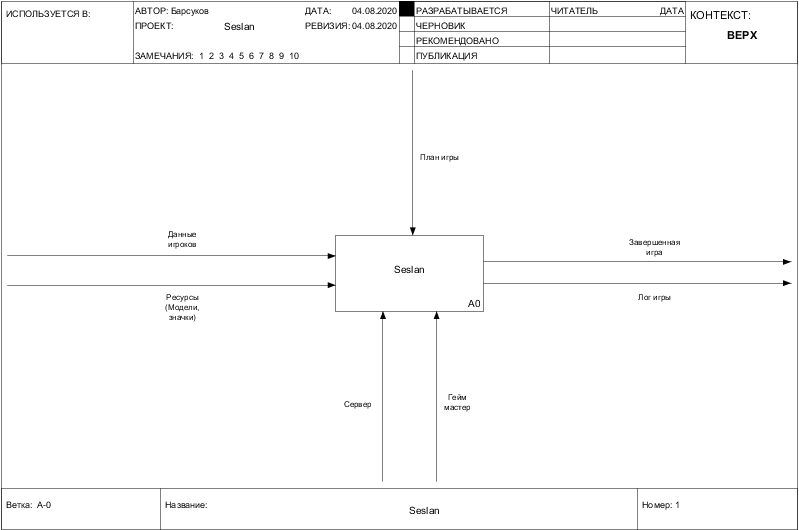
\includegraphics[width=0.7\linewidth]{src/Idef0/01_A-0}
		\caption{}
		\label{fig:01a-0}
	\end{figure}
	
	% TODO: \usepackage{graphicx} required
	\begin{figure}[H]
		\centering
		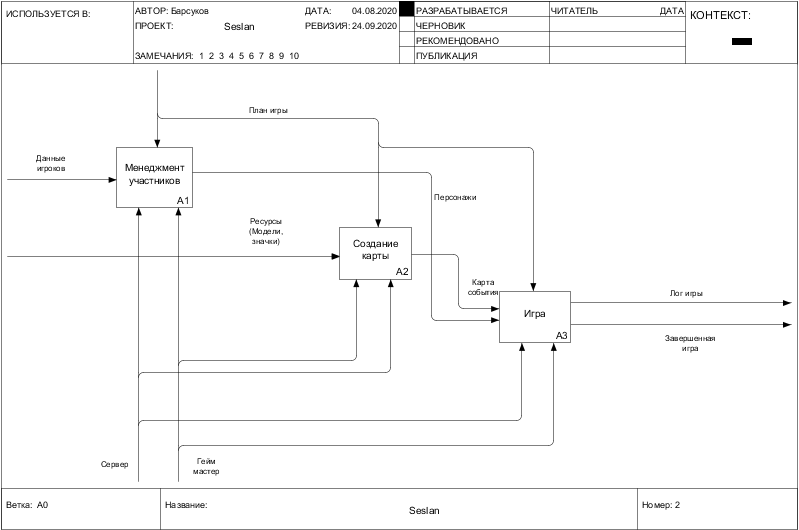
\includegraphics[width=0.7\linewidth]{src/Idef0/02_A0}
		\caption{}
		\label{fig:02a0}
	\end{figure}
	
	% TODO: \usepackage{graphicx} required
	\begin{figure}[H]
		\centering
		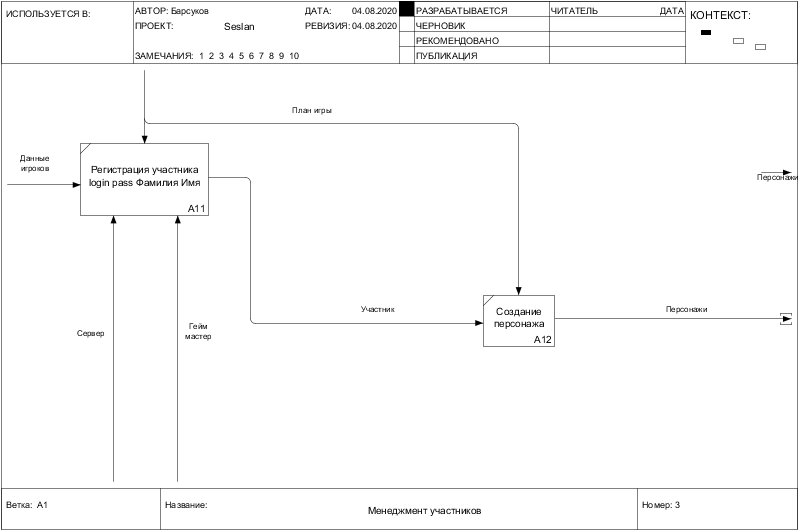
\includegraphics[width=0.7\linewidth]{src/Idef0/03_A1}
		\caption{}
		\label{fig:03a1}
	\end{figure}
	
	% TODO: \usepackage{graphicx} required
	\begin{figure}[H]
		\centering
		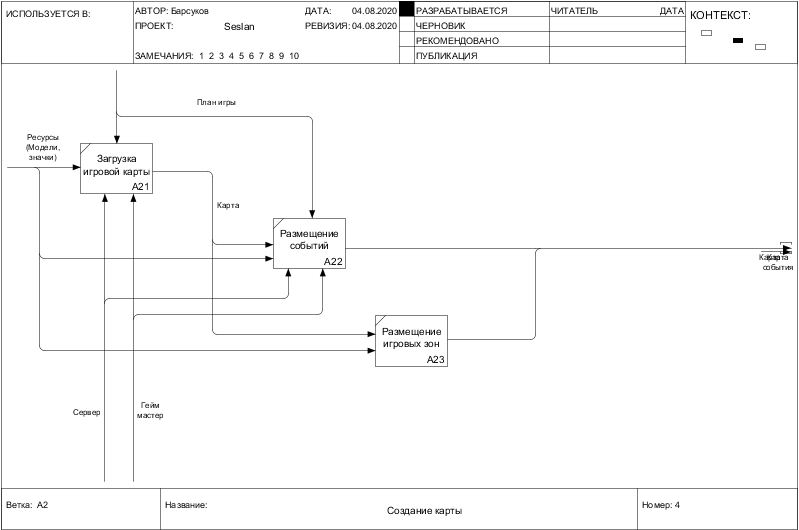
\includegraphics[width=0.7\linewidth]{src/Idef0/04_A2}
		\caption{}
		\label{fig:04a2}
	\end{figure}

	% TODO: \usepackage{graphicx} required
	\begin{figure}[H]
		\centering
		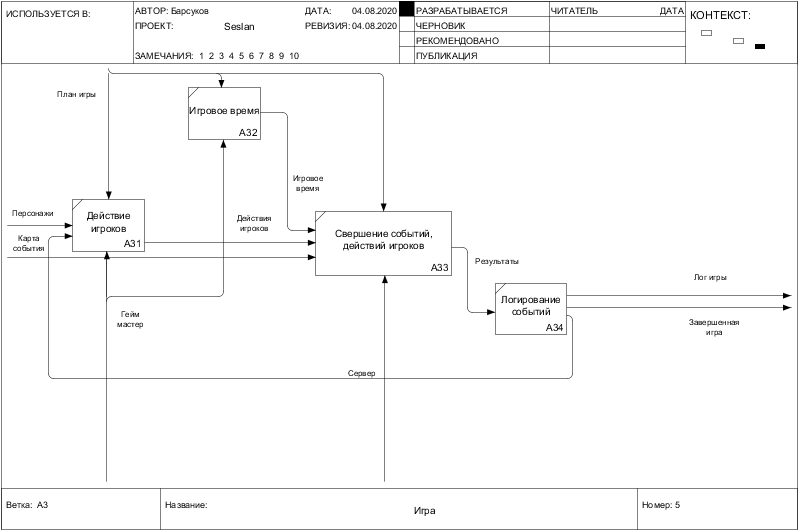
\includegraphics[width=0.7\linewidth]{src/Idef0/05_A3}
		\caption{}
		\label{fig:05a3}
	\end{figure}
	
\subsection{ER}
	
	% TODO: \usepackage{graphicx} required
	\begin{figure}[H]
		\centering
		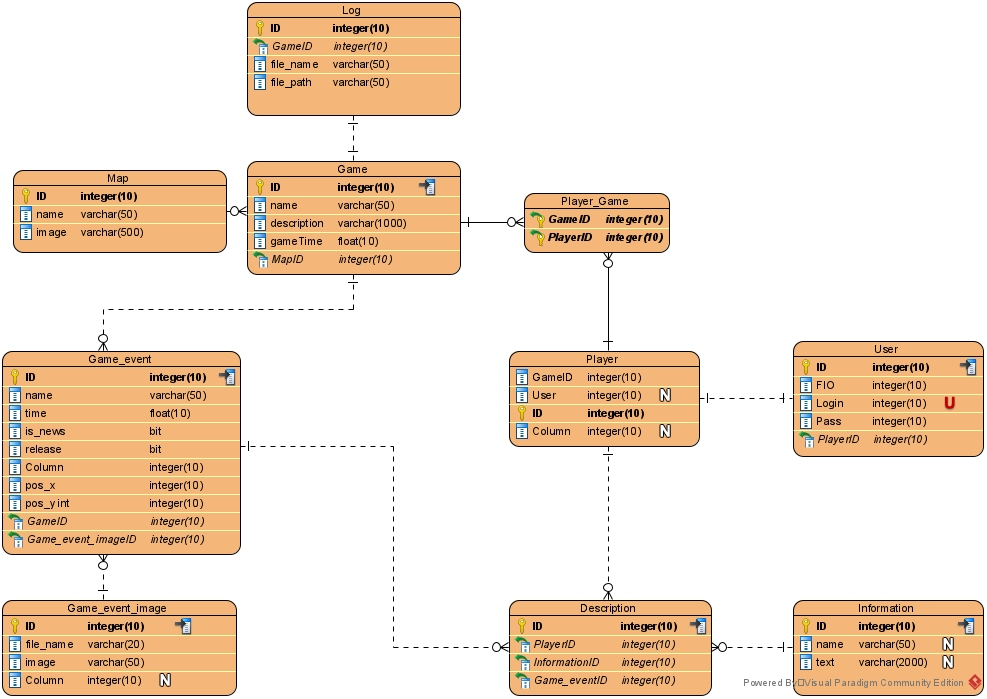
\includegraphics[width=0.7\linewidth]{src/ER}
		\caption{ER диаграмма}
		\label{fig:er}
	\end{figure}
	
	